\documentclass[../main.tex]{subfiles}

\begin{document}



\chapter{General Linear Least-Squares and Nonlinear Regression}
\textbf{CHAPTER OBJECTIVES}

\noindent This chapter takes the concept of fitting a straight line and extends it to (a) fitting a polynomial and (b) fitting a variable that is a linear function of two or more independent variables. We will then show how such applications can be generalized and applied to a broader group of problems. Finally, we will illustrate how optimization techniques can be used to implement nonlinear regression. Specific objectives and topics covered are

\begin{itemize}
	\item Knowing how to implement polynomial regression.
	\item Knowing how to implement multiple linear regression. 
	\item Understanding the formulation of the general linear least-squares model.
	\item Understanding how the general linear least-squares model can be solved with MATLAB using either the normal equations or left division.
	\item Understanding how to implement nonlinear regression with optimization techniques.
\end{itemize}


\label{cha:cha_P_15_1}
\section{POLYNOMIAL REGRESSION}
\noindent In Chap.14, a procedure was developed to derive the equation of a straight line using the least-squares criterion. Some data, although exhibiting a marked pattern such as seen in Fig. 15.1, are poorly represented by a straight line. For these cases, a curve would be better suited to fit the data. As discussed in Chap. 14, one method to accomplish this objective is to use transformations. Another alternative is to fit polynomials to the data using \emph{polynomial regression}.

The least-squares procedure can be readily extended to fit the data to a higher-order polynomial. For example,  suppose that we fit a second-order polynomial or quadratic:

\begin{equation}
	\tag{15.1}
	y = a_0 + a_1x + a_2x^2 + e
\end{equation}

\begin{wrapfigure}{l}{0.25\textwidth}
    \centering
    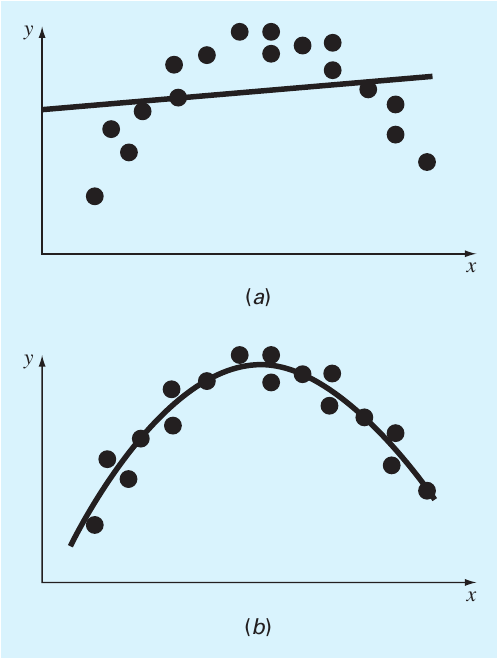
\includegraphics[width=0.25\textwidth]{fig_15_1}
   \caption{\textsf{(a) Data that are ill-suited for linear least-squares regression. (b) Indication that a parabola is preferable.}}
   \label{fig:fig_15_1}
\end{wrapfigure}

\noindent For this case the sum of the squares of the residuals is

\begin{equation}
	\tag{15.2}
	S_r = \sum^n_{i=1}(y_i - a_0 - a_1x_i - a_2x^2_i)^2
\end{equation}

To generate the least-squares fit, we take the derivative of Eq. (15.2) with respect to each of the unknown coefficients of the polynomial, as in

\begin{equation}
	\notag
	\frac{\partial S_r}{\partial a_0} = -2 \sum (y_i -a_0 -a_1x_i - a_2x_i^2)
\end{equation}

\begin{equation}
	\notag
	\frac{\partial S_r}{\partial a_1} = -2 \sum x_i (y_i -a_0 -a_1x_i - a_2x_i^2)
\end{equation}

\begin{equation}
	\notag
	\frac{\partial S_r}{\partial a_2} = -2 \sum x_i^2 (y_i -a_0 -a_1x_i - a_2x_i^2)
\end{equation}

\noindent These equations can be set equal to zero and rearranged to develop the following set of normal equations:

\begin{equation}
	\notag
	(n)a_0 + (\sum x_i) a_1 + (\sum x^2_i) a_2 = \sum y_i
\end{equation}

\begin{equation}
	\notag
	(\sum x_i)a_0 + (\sum x_i ^ 2) a_1 + (\sum x^3_i) a_2 = \sum x_i y_i
\end{equation}

\begin{equation}
	\notag
	(\sum x_i^2)a_0 + (\sum x_i ^ 3) a_1 + (\sum x^4_i) a_2 = \sum x_i^2 y_i
\end{equation}

\noindent where all summations are from $i = 1$ through $n$. Note that the preceding three equations are linear and have three unknowns: $a_0$ , $a_1$, and $a_2$. The coefficients of the unknowns can be calculated directly from the observed data.

For this case, we see that the problem of determining a least-squares second-order polynomial is equivalent to solving a system of three simultaneous linear equations. The two-dimensional case can be easily extended to an $m$th-order polynomial as in

\begin{equation}
	\notag
	y = a_0 + a_1 x + a_2 x^2 + \cdots + a_m x^m + e
\end{equation}

The foregoing analysis can be easily extended to this more general case. Thus, we can recognize that determining the coefficients of an $m$th-order polynomial is equivalent to solving a system of $m + 1$ simultaneous linear equations. For this case, the standard error is formulated as

\begin{equation}
	\tag{15.3}
	s_{y/x} = \sqrt{\frac{S_r}{n - (m + 1)}}
\end{equation}

This quantity is divided by $n - (m + 1)$ because $(m + 1)$ data-derived coefficients - $a_0, a_1, ..., a_m$ - were used to compute $S_r$; thus, we have lost $m + 1$ degrees of freedom. In addition to the standard error, a coefficient of determination can also be computed for polynomial regression with Eq. (14.20).

\begin{example} Polynomial Regression

    \textbf{Problem Statement.}\quad Fit a second-order polynomial to the data in the first two columns
	of Table 15.1.

	\textbf{TABLE 15.1} \quad Computations for an error analysis of the quadratic least-squares fit.

	\begin{tabular}{l c c c c c c c c c c}
		$x_i$ & $y_i$ & $(y_i - \bar{y})^2$ & $(y_i - a_0 - a_1 x_i - a_2 x_i^2 )^2$ \\
		0 &  2.1 &  544.44 &  0.14332 \\
		1 &	 7.7 &  314.47 &  1.00286 \\
		2 &  13.6 &  140.03 &  1.08160 \\
		3 &  27.2 &  3.12 &  0.80487 \\
		4 &  40.9 &  239.22 &  0.61959 \\
		5 &  61.1 &  1272.11 &  0.09434 \\
		$\sum$ & 152.6 &  2513.39 &  3.74657
  	\end{tabular}

	\noindent\textbf{Solution.}\quad The following can be computed from the data:
$$
	\begin{matrix}
		m = 1 & \sum x_i = 15 & \sum x^4_i = 979 \\
		n= 6 & \sum y_i = 152.6 & \sum x_i y_i = 585.6 \\
		\bar{x} = 2.5 & \sum x^2_i = 55 & \sum x^2_i y_i = 2488.8 \\
		\bar{y} = 25.443 & \sum x^3_i = 225
	\end{matrix}
$$

	\noindent Therefore, the simultaneous linear equations are

	$$
		\begin{bmatrix}
			6 & 15 & 55 \\
			15 & 55 & 225 \\
			55 & 225 & 979
		\end{bmatrix}
		\begin{Bmatrix}
			a_0 \\ a_1 \\ a_2
		\end{Bmatrix}
		=
		\begin{Bmatrix}
			152.6 \\
			585.6 \\
			2488.8
		\end{Bmatrix}
	$$

	\noindent These equations can be solved to evaluate the coefficients. For example, using MATLAB:

	\begin{lstlisting}[numbers=none]
		>> N = [6 15 55;15 55 225;55 225 979];
		>> r = [152.6 585.6 2488.8];
		>> a = N\r

		a =
			2.4786
			2.3593
			1.8607
	\end{lstlisting}

	\noindent Therefore, the least-squares quadratic equation for this case is

	$$
		y= 2.4786 + 2.3593x + 1.8607x^2
	$$

	\noindent The standard error of the estimate based on the regression polynomial is [Eq. (15.3)]

	$$
		s_{y/x} = \sqrt{\frac{3.74657}{6 - (2 + 1)}} = 1.1175
	$$

	\noindent The coefficient of determination is

	$$
		r^2 = \frac{2513.39 - 3.74657}{2513.39}= 0.99851
	$$

	\noindent and the correlation coefficient is $r$ = 0.99925.

	\begin{figure}[H]
		\centering
		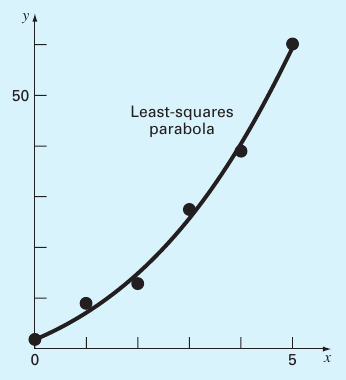
\includegraphics[width=0.5\linewidth]{fig_15_2}
		\caption{\textsf{Fit of a second-order polynomial.}}
		\label{fig:fig_15_2}
	\end{figure}

	These results indicate that 99.851 percent of the original uncertainty has been explained by the model. This result supports the conclusion that the quadratic equation
represents an excellent fit, as is also evident from Fig. 15.2.
\end{example}

\label{cha:cha_P_15_2} % 365
\section{MULTIPLE LINEAR REGRESSION}

\noindent Another useful extension of linear regression is the case where $y$ is a linear function of two or more independent variables. For example, $y$ might be a linear function of $x_1$ and $x_2$, as in

\begin{equation}
	\notag
	y = a_0 + a_1x_1 + a_2x_2+e
\end{equation}

\noindent Such an equation is particularly useful when fitting experimental data where the variable being studied is often a function of two other variables. For this two-dimensional case, the regression ``line'' becomes a ``plane'' (Fig. 15.3).

As with the previous cases, the "best" values of the coefficients are determined by formulating the sum of the squares of the residuals:

\begin{equation}
	\tag{15.4}
	S_r = \sum_{i=1}^n (y_i - a_0 - a_1x_{1,i} - a_2x_{2,i})^2
\end{equation}

\noindent and differentiating with respect to each of the unknown coefficients:

\begin{equation}
	\notag
	\frac{\partial S_r}{\partial a_0} = -2 \sum (y_i -a_0 -a_1x_{1,i} - a_2x_{2,i}^2)
\end{equation}

\begin{equation}
	\notag
	\frac{\partial S_r}{\partial a_1} = -2 \sum x_{1,i} (y_i -a_0 -a_1x_{1,i} - a_2x_{2,i}^2)
\end{equation}

\begin{equation}
	\notag
	\frac{\partial S_r}{\partial a_2} = -2 \sum x_{2,i}^2 (y_i -a_0 -a_1x_{1,i} - a_2x_{2,i}^2)
\end{equation}

\begin{figure}[H]
    \centering
    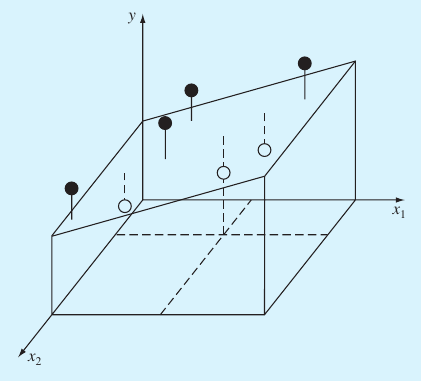
\includegraphics[width=0.5\textwidth]{fig_15_3}
   \caption{\textsf{Graphical depiction of multiple linear regression where y is a linear function of $x_1$ and $x_2$.}}
   \label{fig:fig_15_3}
\end{figure}

\noindent The coefficients yielding the minimum sum of the squares of the residuals are obtained by setting the partial derivatives equal to zero and expressing the result in matrix form as 

\begin{equation} % 366
	\tag{15.5}
	\begin{bmatrix}
		n & \sum x_{1,i} & \sum x_{2,i} \\
		\sum x_{1,i} & \sum x_{1,i}^2 & \sum x_{1,i} x_{2,i} \\
		\sum x_{2,i} & \sum x_{1,i} x_{2,i} & \sum x_{2,i}^2
	\end{bmatrix}
	\begin{Bmatrix}
		a_0 \\ a_1 \\ a_2
	\end{Bmatrix} =
	\begin{Bmatrix}
		\sum y_i \\ \sum x_{1,i} y_i \\ \sum x_{2,i} y_i
	\end{Bmatrix}
\end{equation}

\begin{example} Polynomial Regression

    \textbf{Problem Statement.}\quad The following data were created from the equation $y = 5 + 4x_1 - 3x_2$:

	\begin{tabular}{l c c c c c c c c c c}
		$x_1$ & $x_2$ & $y$ \\
		\hline
		0 & 0 & 5 \\
		2 & 1 & 10 \\
		2.5 & 2 & 9 \\
		1 & 3 & 0 \\
		4 & 6 & 3 \\
		7 & 2 & 27
  	\end{tabular}

	\noindent Use multiple linear regression to fit this data.

	\noindent\textbf{Solution.}\quad The summations required to develop Eq. (15.5) are computed in Table 15.2. Substituting them into Eq. (15.5) gives

	\begin{equation}
		\tag{15.6}
		\begin{bmatrix}
			6 & 16.5 & 14 \\
			16.5 & 76.25 & 48 \\
			14 & 48 & 54
		\end{bmatrix}
		\begin{Bmatrix}
			a_0 \\ a_1 \\ a_2
		\end{Bmatrix}
		=
		\begin{Bmatrix}
			54 \\ 243.5 \\ 100
		\end{Bmatrix}
	\end{equation}

	\noindent which can be solved for

	$$a_0 = 5 \quad a_1 = 4 \quad a_2 = -3$$

	\noindent which is consistent with the original equation from which the data were derived.
\end{example}

The foregoing two-dimensional case can be easily extended to $m$ dimensions, as in

\begin{equation}
	\notag
	y = a_0 + a_1 x_1 + a_2 x_2 + \cdots + a_m x_m + e
\end{equation}

\textbf{TABLE 15.2} \quad Computations required to develop the normal equations for Example 15.2.

\begin{tabular}{c c c c c c c c c c c c c}
	$y$ & $x_1$ & $x_2$ & $x^2_1$ & $x_2^2$ & $x_1 x_2$ & $x_1 y$ & $x_2 y$ \\ 
	\hline
	5 & 0 & 0 & 0 & 0 & 0 & 0 & 0 \\ 
	10 & 2 & 1 & 4 & 1 & 2 & 20 & 10 \\ 
	9 & 2.5 & 2 & 6.25 & 4 & 5 & 22.5 & 18 \\ 
	0 & 1 & 3 & 1 & 9 & 3 & 0 & 0 \\ 
	3 & 4 & 6 & 16 & 36 & 24 & 12 & 18 \\ 
	27 & 7 & 2 & 49 & 4 & 14 & 189 & 54 \\ 
	54 & 16.5 & 14 & 76.25 & 54 & 48 & 243.5 & 100            
\end{tabular}

\noindent where the standard error is formulated as
\begin{equation}
	\notag
	s_{y/x} = \sqrt{\frac{S_r}{n - (m + 1)}}
\end{equation}

\noindent and the coefficient of determination is computed with Eq. (14.20).

Although there may be certain cases where a variable is linearly related to two or more other variables, multiple linear regression has additional utility in the derivation of power equations of the general form 

\begin{equation}
	\notag
	y = a_0 x_1 ^ {a_1} x_2 ^ {a_2} \cdots x_m ^ {a_m}
\end{equation}

\noindent Such equations are extremely useful when fitting experimental data. To use multiple linear regression, the equation is transformed by taking its logarithm to yield

\begin{equation}
	\notag
	\log y = \log a_0 + a_1 \log x_1 + a_2 \log x_2 + \cdots + a_m \log x_m
\end{equation}

\label{cha:cha_P_15_3} %367
\section{GENERAL LINEAR LEAST SQUARES}

\noindent In the preceding pages, we have introduced three types of regression: simple linear, polynomial, and multiple linear. In fact, all three belong to the following general linear least-squares model:

\begin{equation}
	\tag{15.7}
	y = a_0 z_0 + a_1 z_1 + a_2 + z_2 + \cdots + a_m z_m + e
\end{equation}

\noindent where $z_0, z_1, \ldots, z_m$ are $m + 1$ basis functions. It can easily be seen how simple linear and multiple linear regression fall within this model-that is, $z_0 = 1, z_1 = x_1, z_2 = x_2, \ldots, z_m = xm$. Further, polynomial regression is also included if the basis functions are simple monomials as in $z_0 = 1, z_1 = x, z_2 = x^2, \ldots, z_m = x^m$.

Note that the terminology ``linear'' refers only to the model's dependence on its
parameters-that is, the $a$'s. As in the case of polynomial regression, the functions themselves can be highly nonlinear. For example, the $z$'s can be sinusoids, as in

\begin{equation}
	\notag
	y = a_0 + a_1 \cos (\omega x) + a_2 sin (\omega x)
\end{equation}

\noindent Such a format is the basis of \textit{Fourier analysis}

On the other hand, a simple-looking model such as

\begin{equation}
	\notag
	y = a_0 (1- e^{-a_1 x})
\end{equation}

\noindent is truly nonlinear because it cannot be manipulated into the format of Eq. (15.7).

Equation (15.7) can be expressed in matrix notation as

\begin{equation}
	\tag{15.8}
	{y} = [Z] {a} + {e}
\end{equation}

\noindent where $[Z]$ is a matrix of the calculated values of the basis functions at the measured values of the independent variables:

\begin{equation}
	\notag
	\begin{bmatrix}
		z_{01} & z_{11} & \cdots & z_{m1} \\ 
		z_{02} & z_{12} & \cdots & z_{m2} \\ 
		\vdots & \vdots &        & \vdots \\ 
		z_{0n} & z_{1n} & \cdots & z_{mn}
	\end{bmatrix}
\end{equation}

\noindent where $m$ is the number of variables in the model and $n$ is the number of data points. Because $n \geqslant  m + 1$, you should recognize that most of the time, $[Z]$ is not a square matrix.

The column vector ${y}$ contains the observed values of the dependent variable:

\begin{equation}
	\notag
	{y}^T = \lfloor y_1 \quad  y_2 \quad \cdots \quad y_n \rfloor 
\end{equation}

\noindent The column vector ${a}$ contains the unknown coefficients:

\begin{equation}
	\notag
	{a}^T = \lfloor a_1 \quad  a_2 \quad \cdots \quad a_m \rfloor 
\end{equation}

\noindent and the column vector ${e}$ contains the residuals:

\begin{equation}
	\notag
	{e}^T = \lfloor e_1 \quad  e_2 \quad \cdots \quad e_n \rfloor 
\end{equation}

The sum of the squares of the residuals for this model can be defined as

\begin{equation}
	\tag{15.9}
	S_r = \sum^n_{i=1} {(y_i - \sum^m_{j=0} a_j z_{ji})}^2
\end{equation}

\noindent This quantity can be minimized by taking its partial derivative with respect to each of the
coefficients and setting the resulting equation equal to zero. The outcome of this process is
the normal equations that can be expressed concisely in matrix form as

\begin{equation}
	\tag{15.10}
	[{[Z]}^T [Z]] \{a\} = \{{[Z]}^T \{y\}\}
\end{equation}

\noindent It can be shown that Eq. (15.10) is, in fact, equivalent to the normal equations developed
previously for simple linear, polynomial, and multiple linear regression.

The coefficient of determination and the standard error can also be formulated in terms
of matrix algebra. Recall that $r^2$ is defined as

\begin{equation}
	\notag
	r^2 = \frac{S_t - S_r}{S_t} = 1 - \frac{S_r}{S_t}
\end{equation}

\noindent Substituting the definitions of $S_r$ and $S_t$ gives

\begin{equation}
	\notag
	r^2 = 1 - \frac{\sum {(y_i - \hat{y}_i)} ^ 2}{\sum {(y_i - \bar{y}_i)} ^ 2}
\end{equation}

\noindent where $\hat{y} =$ the prediction of the least-squares fit. The residuals between the best-fit curve and the data, $y_i - \hat{y}$, can be expressed in vector form as

\begin{equation}
	\notag
	\{y\} - [Z] \{a\}
\end{equation}

Matrix algebra can then be used to manipulate this vector to compute both the coefficient of determination and the standard error of the estimate as illustrated in the following example.

\begin{example} Polynomial Regression with MATLAB

    \textbf{Problem Statement.}\quad Repeat Example 15.1, but use matrix operations as described in this
	section.

	\noindent\textbf{Solution.}\quad First, enter the data to be fit

	\begin{lstlisting}[numbers=none]
		>> x = [0 1 2 3 4 5]';
		>> y = [2.1 7.7 13.6 27.2 40.9 61.1]';
	\end{lstlisting}

	\noindent Next, create the [Z] matrix:

	\begin{lstlisting}[numbers=none]
		>> Z = [ones(size(x)) x x.^2]
		Z = 
			1  0  0 
			1  1  1 
			1  2  4 
			1  3  9 
			1  4 16 
			1  5 25
	\end{lstlisting}

	\noindent We can verify that [Z]$^T$ [Z] results in the coefficient matrix for the normal equations:

	\begin{lstlisting}[numbers=none]
		>> Z'*Z
		ans = 
			 6  15    55 
			15  55   225 
			55  225  979
	\end{lstlisting}

	\noindent This is the same result we obtained with summations in Example 15.1. We can solve for the	coefficients of the least-squares quadratic by implementing Eq. (15.10):

	\begin{lstlisting}[numbers=none]
		>> a = (Z'*Z)\(Z'*y)
		ans =
			2.4786
			2.3593
			1.8607
	\end{lstlisting}

	\noindent In order to compute $r^2$ and $s_{y/x}$, first compute the sum of the squares of the residuals:

	\begin{lstlisting}[numbers=none]
		>> Sr = sum((y-Z*a).^2)
		Sr =
			3.7466
	\end{lstlisting}

	\noindent Then $r^2$ can be computed as

	\begin{lstlisting}[numbers=none]
		>> r2 = 1-Sr/sum((y-mean(y)).^2)
		r2 =
			0.9985
	\end{lstlisting}

	\noindent and $s_{y/x}$ can be computed as

	\begin{lstlisting}[numbers=none]
		>> syx = sqrt(Sr/(length(x)-length(a)))
		syx =
			1.1175
	\end{lstlisting}
\end{example}

Our primary motivation for the foregoing has been to illustrate the unity among the
three approaches and to show how they can all be expressed simply in the same matrix notation. It also sets the stage for the next section where we will gain some insights into the
preferred strategies for solving Eq. (15.10). The matrix notation will also have relevance
when we turn to nonlinear regression in Section 15.5.

\bigskip
\label{cha:cha_P_15_4} %370
\section{QR FACTORIZATION AND THE BACKSLASH OPERATOR}

\noindent Generating a best fit by solving the normal equations is widely used and certainly adequate
for many curve-fitting applications in engineering and science. 
It must be mentioned, however, that the normal equations can be ill-conditioned and hence sensitive to roundoff errors.

Two more advanced methods, QR \textit{factorization} and \textit{singular value decomposition}, are
more robust in this regard. Although the description of these methods is beyond the scope
of this text, we mention them here because they can be implemented with MATLAB.

Further, QR factorization is automatically used in two simple ways within MATLAB.
First, for cases where you want to fit a polynomial, the built-in \texttt{polyfit} function automatically uses QR factorization to obtain its results.

Second, the general linear least-squares problem can be directly solved with the backslash operator. Recall that the general model is formulated as Eq. (15.8)

\begin{equation}
	\tag{15.11}
	\{y\} = [Z] \{a\}
\end{equation}

In Section 10.4, we used left division with the backslash operator to solve systems of linear algebraic equations where the number of equations equals the number of unknowns $(n = m)$.
For Eq. (15.8) as derived from general least squares, the number of equations is greater than
the number of unknowns $(n > m)$. Such systems are said to be \textit{overdetermined}. When
MATLAB senses that you want to solve such systems with left division, it automatically uses
QR factorization to obtain the solution. The following example illustrates how this is done.

\begin{example} Implementing Polynomial Regression with \texttt{polyfit} and Left Division

    \textbf{Problem Statement.}\quad Repeat Example 15.3, but use the built-in \texttt{polyfit} function and
	left division to calculate the coefficients.

	\noindent\textbf{Solution.}\quad As in Example 15.3, the data can be entered and used to create the [Z] matrix
	as in

	\begin{lstlisting}[numbers=none]
		>> x = [0 1 2 3 4 5]';
		>> y = [2.1 7.7 13.6 27.2 40.9 61.1]';
		>> Z = [ones(size(x)) x x.^2];
	\end{lstlisting}

	\noindent The \texttt{polyfit} function can be used to compute the coefficients:

	\begin{lstlisting}[numbers=none]
		>> a = polyfit(x,y,2)
		a =
			1.8607
			2.3593
			2.4786
	\end{lstlisting}

	The same result can also be calculated using the backslash:

	\begin{lstlisting}[numbers=none]
		>> a = Z\y
		a =
			2.4786
			2.3593
			1.8607	
	\end{lstlisting}

	\noindent As just stated, both these results are obtained automatically with QR factorization.
\end{example}

\bigskip
\label{cha:cha_P_15_5} %370
\section{NONLINEAR REGRESSION}

\noindent There are many cases in engineering and science where nonlinear models must be fit to
data. In the present context, these models are defined as those that have a nonlinear dependence on their parameters. For example,

\begin{equation}
	\tag{15.12}
	y = a_0 (1 - e^{-a_1 x}) + e
\end{equation}

\noindent This equation cannot be manipulated so that it conforms to the general form of Eq. (15.7).

As with linear least squares, nonlinear regression is based on determining the values
of the parameters that minimize the sum of the squares of the residuals. However, for the
nonlinear case, the solution must proceed in an iterative fashion.

There are techniques expressly designed for nonlinear regression. For example, the
Gauss-Newton method uses a Taylor series expansion to express the original nonlinear
equation in an approximate, linear form. Then least-squares theory can be used to obtain
new estimates of the parameters that move in the direction of minimizing the residual.
Details on this approach are provided elsewhere (Chapra and Canale, 2010).

An alternative is to use optimization techniques to directly determine the least-squares
fit. For example, Eq. (15.12) can be expressed as an objective function to compute the sum
of the squares:

\begin{equation}
	\tag{15.13}
	f(a_0, a_1) = \sum^n_{i=1} {[y_i - a_0 (1 - e ^ {-a_i x_i})]} ^ 2
\end{equation}

An optimization routine can then be used to determine the values of $a_0$ and $a_1$ that minimize the function.

As described previously in Section 7.3.1, MATLAB's \texttt{fminsearch} function can be used for this purpose. It has the general syntax

\begin{lstlisting}[numbers=none] 
	[x, fval] = fminsearch(fun,x0,options,p1,p2,...)
\end{lstlisting}

\noindent where $x = a$ vector of the values of the parameters that minimize the function \texttt{fun, fval} = the value of the function at the minimum, \texttt{x0 = }a vector of the initial guesses for the parameters, \texttt{options} = a structure containing values of the optimization parameters as created with the \texttt{optimset} function (recall Sec. 6.5), and \texttt{p1, p2, }etc. = additional arguments that are passed to the objective function. 
Note that if \texttt{options} is omitted, MATLAB uses default values that are reasonable for most problems. If you would like to pass additional arguments (\texttt{p1, p2, }\dots), but do not want to set the options, use empty brackets \texttt{[]} as a place holder.

\begin{example} Nonlinear Regression with MATLAB

    \textbf{Problem Statement.}\quad  Recall that in Example 14.6, we fit the power model to data from
	Table 14.1 by linearization using logarithms. This yielded the model:

	$$
		F = 0.2741 v ^{1.942}
	$$

	\noindent Repeat this exercise, but use nonlinear regression. Employ initial guesses of 1 for the
	coefficients.

	\noindent\textbf{Solution.}\quad First, an M-file function must be created to compute the sum of the squares.
	The following file, called \texttt{fSSR.m}, is set up for the power equation:

	\begin{lstlisting}[numbers=none]
		function f = fSSR(a,xm,ym)
		yp = a(1)*xm.^a(2);
		f = sum((ym-yp).^2);
	\end{lstlisting}

	\noindent In command mode, the data can be entered as

	\begin{lstlisting}[numbers=none]
		>> x = [10 20 30 40 50 60 70 80];
		>> y = [25 70 380 550 610 1220 830 1450];
	\end{lstlisting}

	\noindent The minimization of the function is then implemented by

	\begin{lstlisting}[numbers=none]
		>> fminsearch(@fSSR, [1, 1], [], x, y)
		ans=
			2.5384
			1.4359	
	\end{lstlisting}

	\noindent The best-fit model is therefore

	$$
		F = 2.5384 v^ {1.4359}
	$$

	Both the original transformed fit and the present version are displayed in Fig. 15.4.
	Note that although the model coefficients are very different, it is difficult to judge which fit
	is superior based on inspection of the plot.

	This example illustrates how different best-fit equations result when fitting the same
	model using nonlinear regression versus linear regression employing transformations. This
	is because the former minimizes the residuals of the original data whereas the latter minimizes the residuals of the transformed data.

	\begin{figure}[H]
		\centering
		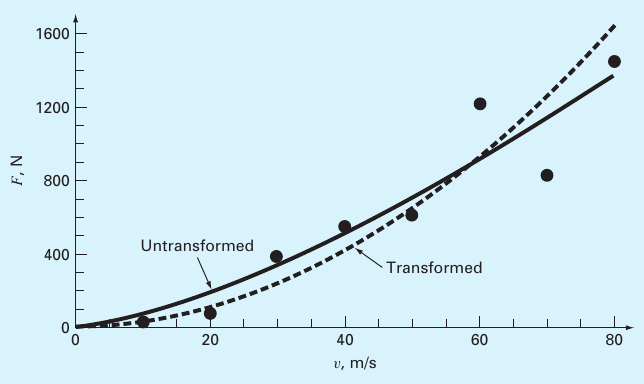
\includegraphics[width=0.5\linewidth]{fig_15_4}
		\caption{\textsf{Comparison of transformed and untransformed model fits for force versus velocity data from
		Table 14.1.}}
		\label{fig:fig_15_4}
	\end{figure}
\end{example}


\section[CASE STUDY: FITTING EXPERIMENTAL DATA]{CASE STUDY: FITTING EXPERIMENTAL DATA}
\noindent\textbf{Background.} \quad As mentioned at the end of Section 15.2, although there are many cases where a variable is linearly related to two or more other variables, multiple linear regression has additional utility in the derivation of multivariable power equations of the general form

\begin{equation}
	\tag{15.14}
	y = a_0 x_1^{a_1} x_2^{a_2} \cdots x_m^{a_m} 
\end{equation}

\noindent Such equations are extremely useful when fitting experimental data. To do this, the equation is transformed by taking its logarithm to yield

\begin{equation}
	\tag{15.15}
	\log y = \log a_0 + a_1 \log x_1 + a_2 \log x_2 \cdots + a_m \log x_m
\end{equation}

\noindent Thus, the logarithm of the dependent variable is linearly dependent on the logarithms of the independent variables.

A simple example relates to gas transfer in natural waters such as rivers, lakes, and estuaries. In particular, it has been found that the mass-transfer coefficient of dissolved oxygen $K_L$ (m/d) is related to a river's mean water velocity $U$ (m/s) and depth $H$ (m) by

\begin{equation}
	\tag{15.16}
	K_L = a_0 U^{a_1} H^{a_2}
\end{equation}

\noindent Taking the common logarithm yields

\begin{equation}
	\tag{15.17}
	\log K_L = \log a_0 + a_1 \log U + a_2 \log H
\end{equation}

The following data were collected in a laboratory flume at a constant temperature of 20 $^\circ$C:

\begin{tabular}{l c c c c c c c c c}
	$U$ & 0.5 & 2 & 10 & 0.5 & 2 & 10 & 0.5 & 2 & 10 \\
	$H$ & 0.15 & 0.15 & 0.15 & 0.3 & 0.3 & 0.3 & 0.5 & 0.5 & 0.5 \\
	$K_L$ & 0.48 & 3.9 & 57 & 0.85 & 5 & 77 & 0.8 & 9 & 92
\end{tabular}

\noindent Use these data and general linear least squares to evaluate the constants in Eq. (15.16).

\noindent Solution. In a similar fashion to Example 15.3, we can develop a script to assign the
data, create the $[Z]$ matrix, and compute the coefficients for the least-squares fit:

\begin{lstlisting}[numbers=none]
	% Compute best fit of transformed values
	clc; format short g
	U=[0.5 2 10 0.5 2 10 0.5 2 10]';
	H=[0.15 0.15 0.15 0.3 0.3 0.3 0.5 0.5 0.5]';
	KL=[0.48 3.9 57 0.85 5 77 0.8 9 92]';
	logU=log10(U);logH=log10(H);logKL=log10(KL);
	Z=[ones(size(logKL)) logU logH];
	a=(Z'*Z)\(Z'*logKL)
\end{lstlisting}

\noindent with the result:

\begin{lstlisting}[numbers=none]
	a =
		0.57627
		1.562
		0.50742
\end{lstlisting}

\noindent Therefore, the best-fit model is

\begin{equation}
	\notag
	\log K_L = 0.57627 + 1.562 \log U + 0.50742 \log H
\end{equation}

\noindent or in the untransformed form (note, $a_0 = 10^{0.57627} = 3.7694$),

\begin{equation}
	\notag
	K_L = 3.7694 U^{1.560} H ^ {0.5074}
\end{equation}

\noindent The statistics can also be determined by adding the following lines to the script:

\begin{lstlisting}[numbers=none]
	% Compute fit statistics
	Sr=sum((logKL-Z*a).^2)
	r2=1-Sr/sum((logKL-mean(logKL)).^2)
	syx=sqrt(Sr/(length(logKL)-length(a)))
	Sr =
		0.024171
	r2 =
		0.99619
	syx =
		0.063471
\end{lstlisting}

Finally, plots of the fit can be developed. The following statements display the model
predictions versus the measured values for $K_L$. Subplots are employed to do this for both
the transformed and untransformed versions.

\begin{lstlisting}[numbers=none]
	%Generate plots
	clf
	KLpred=10^a(1)*U.^a(2).*H.^a(3);
	KLmin=min(KL);KLmax=max(KL);
	dKL=(KLmax-KLmin)/100;
	KLmod=[KLmin:dKL:KLmax];
	subplot(1,2,1)
	loglog(KLpred,KL,'ko',KLmod,KLmod,'k-')
	axis square,title('(a) log-log plot')
	legend('model prediction','1:1
	line','Location','NorthWest')
	xlabel('log(K_L) measured'),ylabel('log(K_L) predicted')
	subplot(1,2,2)
	plot(KLpred,KL,'ko',KLmod,KLmod,'k-')
	axis square,title('(b) untransformed plot')
	legend('model prediction','1:1
	line','Location','NorthWest')
	xlabel('K_L measured'),ylabel('K_L predicted')
\end{lstlisting}

\noindent The result is shown in Fig. 15.5.

\begin{figure}[H]
	\centering
	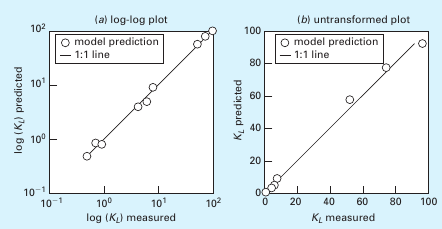
\includegraphics[width=0.5\linewidth]{fig_15_5}
	\caption{\textsf{Plots of predicted versus measured values of the oxygen mass-transfer coefficient as computed with multiple regression. Results are shown for (a) log transformed and (b) untransformed cases. The 1:1 line, which indicates a perfect correlation, is superimposed on both plots.}}
	\label{fig:fig_15_5}
\end{figure}


\setlength{\tabcolsep}{3pt}

\noindent\textbf{PROBLEMS}\\

\begin{multicols}{2}
    \noindent\textbf{15.1}  Fit a parabola to the data from Table 14.1. Determine
	the r 2 for the fit and comment on the efficacy of the result.

	\noindent\textbf{15.2} Using the same approach as was employed to derive
	Eqs. (14.15) and (14.16), derive the least-squares fit of the
	following model:

	$$
		y = a_1 x + a_2 x^2 + e
	$$

	\noindent That is, determine the coefficients that result in the leastsquares fit for a second-order polynomial with a zero inter	cept. Test the approach by using it to fit the data from
	Table 14.1.

	\noindent\textbf{15.3} Fit a cubic polynomial to the following data:

	\noindent
	\begin{tabular}{l c c c c c c c c}
		x & 3 & 4 & 5 & 7 & 8 & 9 & 11 & 12 \\
		y & 1.6 & 3.6 & 4.4 & 3.4 & 2.2 & 2.8 & 3.8 & 4.6
	\end{tabular}

	\noindent Along with the coefficients, determine $r^2$ and $s_{y/x}$.

	\noindent\textbf{15.4} Develop an M-file to implement polynomial regression. Pass the M-file two vectors holding the $x$ and $y$
	values along with the desired order $m$. Test it by solving
	Prob. 15.3.

	\noindent\textbf{15.5}  For the data from Table P15.5, use polynomial
	regression to derive a predictive equation for dissolved
	oxygen concentration as a function of temperature for the
	case where the chloride concentration is equal to zero.
	Employ a polynomial that is of sufficiently high order that
	the predictions match the number of significant digits displayed in the table.

	\noindent\textbf{15.6} Use multiple linear regression to derive a predictive
	equation for dissolved oxygen concentration as a function of
	temperature and chloride based on the data from Table P15.5.
	Use the equation to estimate the concentration of dissolved
	oxygen for a chloride concentration of 15 g/L at $T = 12$ $^\circ$C.
	Note that the true value is 9.09 mg/L. Compute the percent

	\noindent\textbf{TABLE P15.5} Dissolved oxygen concentration in water as a function of temperature ($^\circ$C) and chloride concentration (g/L).

	\noindent
	\begin{tabular}{c c c c}
		T, $^\circ$C & c = 0 g/L & c = 10 g/L & c = 20 g/L \\
		\hline
		0 & 14.6 & 12.9 & 11.4 \\
		5 & 12.8 & 11.3 & 10.3 \\
		10 & 11.3 & 10.1 & 8.96 \\
		15 & 10.1 & 9.03 & 8.08 \\
		20 & 9.09 & 8.17 & 7.35 \\
		25 & 8.26 & 7.46 & 6.73 \\
		30 & 7.56 & 6.85 & 6.20
	\end{tabular}

	\noindent relative error for your prediction. Explain possible causes for
	the discrepancy.

	\noindent\textbf{15.7} As compared with the models from Probs. 15.5 and
	15.6, a somewhat more sophisticated model that accounts
	for the effect of both temperature and chloride on dissolved oxygen saturation can be hypothesized as being of
	the form

	$$
		o = f_3 (T ) + f_1(c)
	$$

	\noindent That is, a third-order polynomial in temperature and a linear
	relationship in chloride is assumed to yield superior results.
	Use the general linear least-squares approach to fit this
	model to the data in Table P15.5. Use the resulting equation
	to estimate the dissolved oxygen concentration for a chloride
	concentration of 15 g/L at $T = 12$ $^\circ$C. Note that the true
	value is 9.09 mg/L. Compute the percent relative error for
	your prediction.

	\noindent\textbf{15.8} Use multiple linear regression to fit

	\noindent
	\begin{tabular}{l c c c c c c c c c c c c}
		\textbf{$x_1$} & 0 & 1 & 1 & 2 & 2 & 3 & 3 & 4 & 4 \\
		\textbf{$x_2$} & 0 & 1 & 2 & 1 & 2 & 1 & 2 & 1 & 2 \\
		\textbf{$y$} & 15.1 & 17.9 & 12.7 & 25.6 & 20.5 & 35.1 & 29.7 & 45.4 & 40.2
	\end{tabular}

	\noindent Compute the coefficients, the standard error of the estimate,
	and the correlation coefficient.

	\noindent\textbf{15.9} The following data were collected for the steady flow of water in a concrete circular pipe:

	\noindent
	\begin{tabular}{c c c c}
		\textbf{Experiment} & \textbf{Diameter, m} & \textbf{Slope, m/m} & \textbf{Flow, m$^3$/s} \\
		1 & 0.3 & 0.001 & 0.04 \\
		2 & 0.6 & 0.001 & 0.24 \\
		3 & 0.9 & 0.001 & 0.69 \\
		4 & 0.3 & 0.01 & 0.13  \\
		5 & 0.6 & 0.01 & 0.82 \\
		6 & 0.9 & 0.01 & 2.38 \\
		7 & 0.3 & 0.05 & 0.31 \\
		8 & 0.6 & 0.05 & 1.95 \\
		9 & 0.9 & 0.05 & 5.66
	\end{tabular}

	\noindent Use multiple linear regression to fit the following model to this data:

	$$
		Q = \alpha_0 D^{\alpha_1} S^{\alpha_2}
	$$

	\noindent where $Q$ = flow, $D$ = diameter, and $S$ = slope.

	\noindent\textbf{15.10} Three disease-carrying organisms decay exponentially in seawater according to the following model:

	$$
		p(t) = Ae^{-1.5t} + Be^{-0.3t} + Ce^{-0.05t}
	$$

	\noindent Estimate the initial concentration of each organism ($A$, $B$,
	and $C$) given the following measurements:

	\noindent
	\begin{tabular}{l c c c c c c c c c}
		\textbf{t} & 0.5 & 1 & 2 & 3 & 4 & 5 & 6 & 7 & 9 \\
		\textbf{p(t)} & 6 & 4.4 & 3.2 & 2.7 & 2 & 1.9 & 1.7 & 1.4 & 1.1
	\end{tabular}

	\noindent\textbf{15.11} The following model is used to represent the effect of
	solar radiation on the photosynthesis rate of aquatic plants:

	$$
		P = P_m \frac{I}{I_{\text{sat}}} e ^ {-\frac{I}{I_{\text{sat}}} + 1}
	$$

	\noindent where $P$ = the photosynthesis rate (mg $m^{-3}$ $d^{-1}$ ),$P_m$ = the
	maximum photosynthesis rate (mg $m^{-3}$ $d^{-1}$ ), $I$ = solar
	radiation ($\mu E m^{-2} s^{-1}$), and $I_{\text{sat}}$ = optimal solar radiation
	($\mu E m^{-2} s^{-1}$). Use nonlinear regression to evaluate $P_m$ and
	$I_{\text{sat}}$ based on the following data:

	\noindent
	\begin{tabular}{l c c c c c c c c c c c c}
		\textbf{I} & 50 & 80 & 130 & 200 & 250 & 350 & 450 & 550 & 700 \\
		\textbf{P} & 99 & 177 & 202 & 248 & 229 & 219 & 173 & 142 & 72
	\end{tabular}

	\noindent\textbf{15.12} The following data are provided

	\noindent
	\begin{tabular}{l c c c c c}
		\textbf{x} & 1 & 2 & 3 & 4 & 5 \\
		\textbf{y} & 2.2 & 2.8 & 3.6 & 4.5 & 5.5
	\end{tabular}

	\noindent Fit the following model to this data using MATLAB and the
	general linear least-squares model

	$$
		y= a + bx + \frac{c}{x}
	$$

	\noindent\textbf{15.13} In Prob. 14.8 we used transformations to linearize
	and fit the following model:

	$$
		y = \alpha_4 x e^{\beta_4 x}
	$$

	\noindent Use nonlinear regression to estimate $\alpha_4$ and $\beta_4$ based on the
	following data. Develop a plot of your fit along with the data.

	\noindent
	\begin{tabular}{l c c c c c c c c c c c c c c}
		\textbf{x}& 0.1& 0.2& 0.4& 0.6& 0.9 &1.3 &1.5 &1.7 &1.8 \\
		\textbf{y}& 0.75 &1.25 &1.45 &1.25& 0.85& 0.55 &0.35& 0.28& 0.18
	\end{tabular}

	\noindent\textbf{15.14}  Enzymatic reactions are used extensively to characterize biologically mediated reactions. The following is an example of a model that is used to fit such reactions:

	$$
		v_0 = \frac{k_m [S]^3}{K + [S]^3}
	$$

	\noindent where $v_0$ = the initial rate of the reaction (M/s), $[S]$ = the substrate concentration (M), and $k_m$ and $K$ are parameters. The following data can be fit with this model:

	\noindent
	\begin{tabular}{c c}
		\textbf{[S], M} & \textbf{$v_0$, M/s} \\
 0.01 &  $6.078 \times 10^{-11}$ \\
0.05 &  $7.595 \times 10^{-9}$ \\
0.1 &  $6.063 \times 10^{-8}$ \\
 0.5 &  $5.788 \times 10^{-6}$ \\
 1 &  $1.737 \times 10^{-5}$ \\
 5 &  $2.423 \times 10^{-5}$ \\
10 &  $2.430 \times 10^{-5}$ \\
50 &  $2.431 \times 10^{-5}$ \\
 100 &  $2.431 \times 10^{-5}$ 
	\end{tabular}

	\noindent \textbf{(a)} Use a transformation to linearize the model and evaluate
the parameters. Display the data and the model fit on a
graph.

\noindent \textbf{(b)} Perform the same evaluation as in \textbf{(a)} but use nonlinear
regression.
 
	\noindent\textbf{15.15} Given the data

	\begin{tabular}{l c c c c c c c c c c }
		\textbf{x} & 5 & 10 & 15 & 20 & 25 & 30 & 35 & 40 & 45 & 50 \\
		\textbf{y} & 17 & 24 & 31 & 33 & 37 & 37 & 40 & 40 & 42 & 41
	\end{tabular}

	\noindent use least-squares regression to fit \textbf{(a)} a straight line, \textbf{(b)} a
	power equation, \textbf{(c)} a saturation-growth-rate equation, and
	\textbf{(d)} a parabola. For \textbf{(b)} and \textbf{(c)}, employ transformations to
	linearize the data. Plot the data along with all the curves. Is
	any one of the curves superior? If so, justify.

	\noindent\textbf{15.16} The following data represent the bacterial growth in a
	liquid culture over of number of days:

	\noindent
	\begin{tabular}{l c c c c c c c c}
		Day & 0 & 4 & 8 & 12 & 16 & 20 \\
		Amount $\times 10^6$ & 67.38 & 74.67 & 82.74 & 91.69 & 101.60 & 112.58
	\end{tabular}

	\noindent Find a best-fit equation to the data trend. Try several
	possibilities—linear, quadratic, and exponential. Determine
   the best equation to predict the amount of bacteria after
   30 days.

   \noindent\textbf{15.17}Dynamic viscosity of water $\mu$ ($10^{-3}$ N $\cdot $ s/m$^2$ ) is related to temperature $T$ ($^\circ$C) in the following manner:

	\noindent
	\begin{tabular}{l c c c c c c}
		$T$ &	0 &	5 &	10 &	20 &	30 &	40 \\
		$\mu$ & 1.787 & 1.519 & 1.307 &	1.002 &	0.7975 & 0.6529
	\end{tabular}
  
	\noindent \textbf{(a)} Plot this data.
	\noindent \textbf{(b)} Use linear interpolation to predict $\mu$ at $T = 7.5$ $^\circ$C.
	\noindent \textbf{(c)} Use polynomial regression to fit a parabola to the data in
order to make the same prediction.

	\noindent\textbf{15.18}  Use the following set of pressure-volume data to find
	the best possible virial constants ($A_1$ and $A_2$) for the following equation of state. $R$ = 82.05 mL atm/gmol K, and $T$ =
	 303 K.

	$$
		\frac{P V}{R T}=1 + \frac{A_1}{V}+\frac{A_2}{V^2} 
	$$
	
	\noindent
	\begin{tabular}{l c c c c }
		\textbf{P (atm)} &		0.985 &		 1.108 &		 1.363 &		 1.631 \\	 
		\textbf{V (mL)} &		 25,000 &		 22,200 &		 18,000 &		 15,000
	\end{tabular}

	\noindent\textbf{15.19} Environmental scientists and engineers dealing with
	the impacts of acid rain must determine the value of the
	ion product of water $K_w$ as a function of temperature. Scientists have suggested the following equation to model this
	relationship:

	$$
		- \log_10 K_w = \frac{a}{T_a} + b \log_10 T_a + c T_a +d
	$$

	\noindent where $T_a$ = absolute temperature (K), and $a$, $b$, $c$, and $d$ are
	parameters. Employ the following data and regression to estimate the parameters with MATLAB. Also, generate a
	plot of predicted $K_w$ versus the data.

	\noindent
	\begin{tabular}{c c}
		T ($^\circ$C) & $K_w$ \\
		0  & $1.164 \times 10^{-15}$ \\
		10 & $2.950 \times 10^{-15}$ \\
		20 & $6.846 \times 10^{-15}$ \\
		30 & $1.467 \times 10^{-14}$ \\
		40 & $2.929 \times 10^{-14}$ \\
	\end{tabular}

	\noindent\textbf{15.20} The distance required to stop an automobile consists
	of both thinking and braking components, each of which is a
	function of its speed. The following experimental data were
	collected to quantify this relationship. Develop best-fit equations for both the thinking and braking components. Use
	these equations to estimate the total stopping distance for a
	car traveling at 110 km/h.

	\begin{tabular}{l c c c c c c} 
		\textbf{Speed, km/h} &  30 &  45 &  60 &  75 &  90 &  120 \\
		\textbf{Thinking, m} &  5.6 &  8.5 &  11.1 &  14.5 &  16.7 &  22.4 \\
		\textbf{Braking, m} &  5.0 &  12.3 &  21.0 &  32.9 &  47.6 &  84.7
	\end{tabular}

	\noindent\textbf{15.21} An investigator has reported the data tabulated below.
	It is known that such data can be modeled by the following
   equation

   $$
	x = e^{(y-b) / a}
   $$

   \noindent where $a$ and $b$ are parameters. Use nonlinear regression to
   determine $a$ and $b$. Based on your analysis predict $y$ at $x = 2.6$.

   \noindent
   \begin{tabular}{l c c c c c }
	\textbf{x} &	1 &	2 &	3 &	4 &	5 \\
	\textbf{y} &	0.5 &	2 &	2.9 &	3.5 &	4
   \end{tabular}

   \noindent\textbf{15.22} It is known that the data tabulated below can be modeled by the following equation

   $$
 	y = ( \frac{a + \sqrt{x}}{b \sqrt{x}})^2  
   $$

   \noindent Use nonlinear regression to determine the parameters $a$ and $b$.
   Based on your analysis predict $y$ at $x = 1.6$.

   \noindent 
   \begin{tabular}{l c c c c c c}
	\textbf{x} &	1 &	2 &	3 &	4 &	5 \\
	\textbf{y} &	0.5 &	2 &	2.9 &	3.5 &	4
   \end{tabular}

   \noindent\textbf{15.23}  An investigator has reported the data tabulated below
   for an experiment to determine the growth rate of bacteria $k$
   (per d), as a function of oxygen concentration $c$ (mg/L). It is
   known that such data can be modeled by the following
   equation:

   $$
 	k = \frac{k_{\text{max}} c^2}{c_s + c^2}  
   $$

   \noindent Use nonlinear regression to estimate $c_s$ and $k_{\text{max}}$ and predict
   the growth rate at $c$ = 2 mg/L.
   
   \begin{tabular}{l c c c c c}
		\textbf{c} &	0.5 &	0.8 &	1.5 &	2.5 &	4 \\
		\textbf{k} &	1.1 &	2.4 &	5.3 &	7.6 &	8.9
   \end{tabular}

   \noindent\textbf{15.24} A material is tested for cyclic fatigue failure whereby
   a stress, in MPa, is applied to the material and the number of
   cycles needed to cause failure is measured. The results are in
   the table below. Use nonlinear regression to fit a power
	model to this data.

	\noindent
	\begin{tabular}{l c c c c c c c}
		\textbf{$N$, cycles} &1 & 10 &100 &1000& 10,000& 100,000& 1,000,000\\
		\textbf{Stress,} \\
		\textbf{MPa} & 1100 & 1000 & 925 & 800 &	625 &	550 &	420
	\end{tabular}

	\noindent\textbf{15.25} The following data shows the relationship between the viscosity of SAE 70 oil and temperature. Use nonlinear regression to fit a power equation to this data.

	\noindent
	\begin{tabular}{l c c c c}
		\textbf{Temperature}, $T$, $^\circ$C 26.67 & 93.33 & 148.89 & 315.56 \\
		\textbf{Viscosity}, $\mu$, N$\cdot$s/m$^2$ 1.35 & 0.085 & 0.012 & 0.00075
	\end{tabular}

	\noindent\textbf{15.26} The concentration of E. \textit{coli} bacteria in a swimming
	area is monitored after a storm:

	\noindent
	\begin{tabular}{l c c c c c c}
		\textbf{t (hr)} &	4 &	8 &	12 &	16 &	20 &	24 \\
		\textbf{c(CFU/100 mL)} &	1590 &	1320 &	1000 &	900 &	650 &	560	   
	\end{tabular}

	\noindent The time is measured in hours following the end of the storm
and the unit CFU is a ``colony forming unit.'' Employ nonlinear regression to fit an exponential model (Eq. 14.22) to
this data. Use the model to estimate \textbf{(a)} the concentration at
the end of the storm ($t = 0$) and \textbf{(b)} the time at which the
concentration will reach 200 CFU/100 mL.

	\noindent\textbf{15.27} Use the following set of pressure-volume data to
	find the best possible virial constants ($A_1$ and $A_2$ ) for the
	equation of state shown below. $R$ = 82.05 mL atm/gmol K
	and $T$ = 303 K.

	$$
		\frac{PV}{RT} = 1 + \frac{A_1}{V} + \frac{A_2}{V^2}
	$$
   
	\noindent
	\begin{tabular}{l c c c c}
		\textbf{P (atm)} & 0.985 & 1.108 & 1.363 & 1.631 \\
		\textbf{V (mL)} & 25,000 & 22,200 & 18,000 & 15,000
	\end{tabular}

	\noindent\textbf{15.28} Three disease-carrying organisms decay exponentially in lake water according to the following model:

	$$
		p(t) = Ae^{-1.5t} + Ae^{-0.3t} + Ae^{-0.05t}
	$$

	\noindent  Estimate the initial population of each organism ($A$, $B$,
	and $C$) given the following measurements:

	\noindent
	\begin{tabular}{l c c c c c c c c c}
		\textbf{t, hr} & 0.5 & 1 & 2 & 3 & 4 & 5 & 6 & 7 & 9 \\
		\textbf{p(t)} & 6.0 & 4.4 & 3.2 & 2.7 & 2.2 & 1.9 & 1.7 & 1.4 & 1.1
	\end{tabular}
\end{multicols}

\end{document}
